\documentclass{article}
\usepackage[utf8]{inputenc}
\usepackage{amsfonts, amsmath, amssymb, amsthm,enumitem}
\usepackage[margin = 1in]{geometry}
\usepackage{graphicx}

%%%THEOREM ENVIRONMENTS%%%
\newtheorem{theorem}{Theorem}
\newtheorem{lemma}{Lemma}
\newtheorem{corollary}{Corollary}
\newtheorem{prop}{Proposition}

\theoremstyle{definition}
\newtheorem{definition}{Definition}
\newtheorem{problem}{Problem}

%%%RESOURCE STATEMENT%%%
\newcommand{\collaborators}[1]{\noindent\textit{For this problem set I collaborated with: Veronika}}
\newcommand{\resources}[1]{\noindent\textit{For this problem set I used the following books/websites: A Walk Through Combinatorics, Bona; An Introduction to the Theory of Numbers, Moser}}

\def\acts{\curvearrowright}

\DeclareMathOperator{\im}{Im}
\DeclareMathOperator{\Stab}{Stab}

\setenumerate[0]{label=(\alph*)} %%makes lists enumerate in (a), (b), ... style

%%%%%%%%%%%%%%%%%%%%%%
%%%%%%%%%%%%%%%%%%%%%%
%%%%%%%%%%%%%%%%%%%%%%
%%%%%%%%%%%%%%%%%%%%%%
%%%%%%%%%%%%%%%%%%%%%%


\title{Combinatorics I HW 1}
\author{Aidan Jalili}
\date{\today}
\begin{document}
\maketitle

%%%%%%%%%%%%%%%%%%%%%%
%%%%%%%%%%%%%%%%%%%%%%
%%%%%%%%%%%%%%%%%%%%%%
%%%%%%%%%%%%%%%%%%%%%%
%%%%%%%%%%%%%%%%%%%%%%

\hrule
\collaborators{[names of collaborators]}

\resources{[titles/links to resources]}
\hrule

%%%%%%%%%%%%%%%%%%%%%%
%%%%%%%%%%%%%%%%%%%%%%
%%%%%%%%%%%%%%%%%%%%%%
%%%%%%%%%%%%%%%%%%%%%%
%%%%%%%%%%%%%%%%%%%%%%



\begin{problem}
\textit{How many odd numbers between 1000 and 9999 have at least 1 even digit?}\\

Another way of asking this question is how many numbers between 1000 and 9999 have all odd digits.\\

First, we look at how many odd numbers there are between 1000 and 9999 total. We know that the first digit
can either be 1,2,3,4,5,6,7,8, or 9. The second digit can be any number between 0 and 9, the third likewise.
Finally, the last digit can either be a 1,3,5,7 or 9. This leave us with the total number of options of:
$9\cdot10\cdot10\cdot5$.\\

Next we can answer how many have all odds. In this case there are 5 possible numbers each digit can be:
1,3,5,7, or 9. This leave us with $5\cdot5\cdot5\cdot5 = 5^4$ possible all odd digit numbers.\\

Therefore the number of these odd numbers that have at least one even digit is:\\

$10^2\cdot9\cdot5-5^4=3875$.\\

\end{problem}

\begin{problem}
    \ \\

    a) $16 \choose 12$\\

    This is the same question we raised in class with picking beer from different brands. There are multiple explanations as to why
    (the robot analogy being one, but also building a bijection from the set of possible choices to the number of subsets of size 12 of a set of size 16).

    b) $5^{12}$\\

    Since order doesn't matter it's just 5 possible choices of beans 12 times.
\end{problem}

\begin{problem}
    \ \\

\end{problem}
We know that ${n\choose k}^2 = {n\choose k} \cdot {n\choose{n-k}}$. Therefore:
\begin{align*}
    &\sum_{n=0}^k {n\choose k}^2 = \sum_{n=0}^k {n\choose k} \cdot {n \choose {n-k}}.\\ 
\end{align*}
This is the same as the number of size $n$ subsets of a set of size $2n$, (the right hand side of the original identity). First
we divide the set of size $2n$ into two equal $n$-size sets. From the first
we pick $k$ elements, From the second, $n-k$. Summing up over all possible ways our pick
can be divided into ``first half'' vs. ``back half'' enables us to count all possible ways our pick of subset of $n$ size 
``divides'' into these two halves. The result should be the same as if we didn't divide the set into halves and just simply picked
the $n$ elements directly from the entire set of size $2n$.
\begin{problem}
Proof that for all $n$ greater than or equal to $2$, $\sum_{k=2}^n k(k-1) {n \choose k} = n(n-1)2^{n-2}$\\

We notice that the right hand side is the number of different ways you can make subsets of a set of size n, where you label two specific elements from that set (e.g. making a committe with a chair and vice chair say). The left hand size is 
the same. The only difference in the two sides is how we count. The right hand, we pick the two elements we guarantee to be in the set (this would correspond to labeling one as chair, and another as vice chair),
and then the number of possible subsets that can be made with the remaining elements. On the left we first calculate the number of ways we can pick a two element subset,
then add that to the number of ways we can pick a three element subset, then so on, all the way up to $n$. For each of these subsets we multiply by the number of different ways we could label a chair and vice chair within that subset.\\
\end{problem}

\begin{problem}
The way I thought of this probem is with graphs. If we think of the five players as being $\mathbb{N}_5$ where I'm using the notation
$\mathbb{N}_x = \{1,2,3,4,...,x\}$ then we can obtain a visual representation of the order they come out in. (Here the representation is that the shortest player is 1, the second shortest 2, etc. So the tallest player is represented by number 5.)\\

If we let the x-axis correspond to the position that player walked out in (e.g. 1st, 2nd, 3rd, etc.) and the y-axis be the player that came out in that position
(e.g. the shortest player, which would be 1, the second shortest, which would be 2, etc.) we can obtain a graph like the following:\\

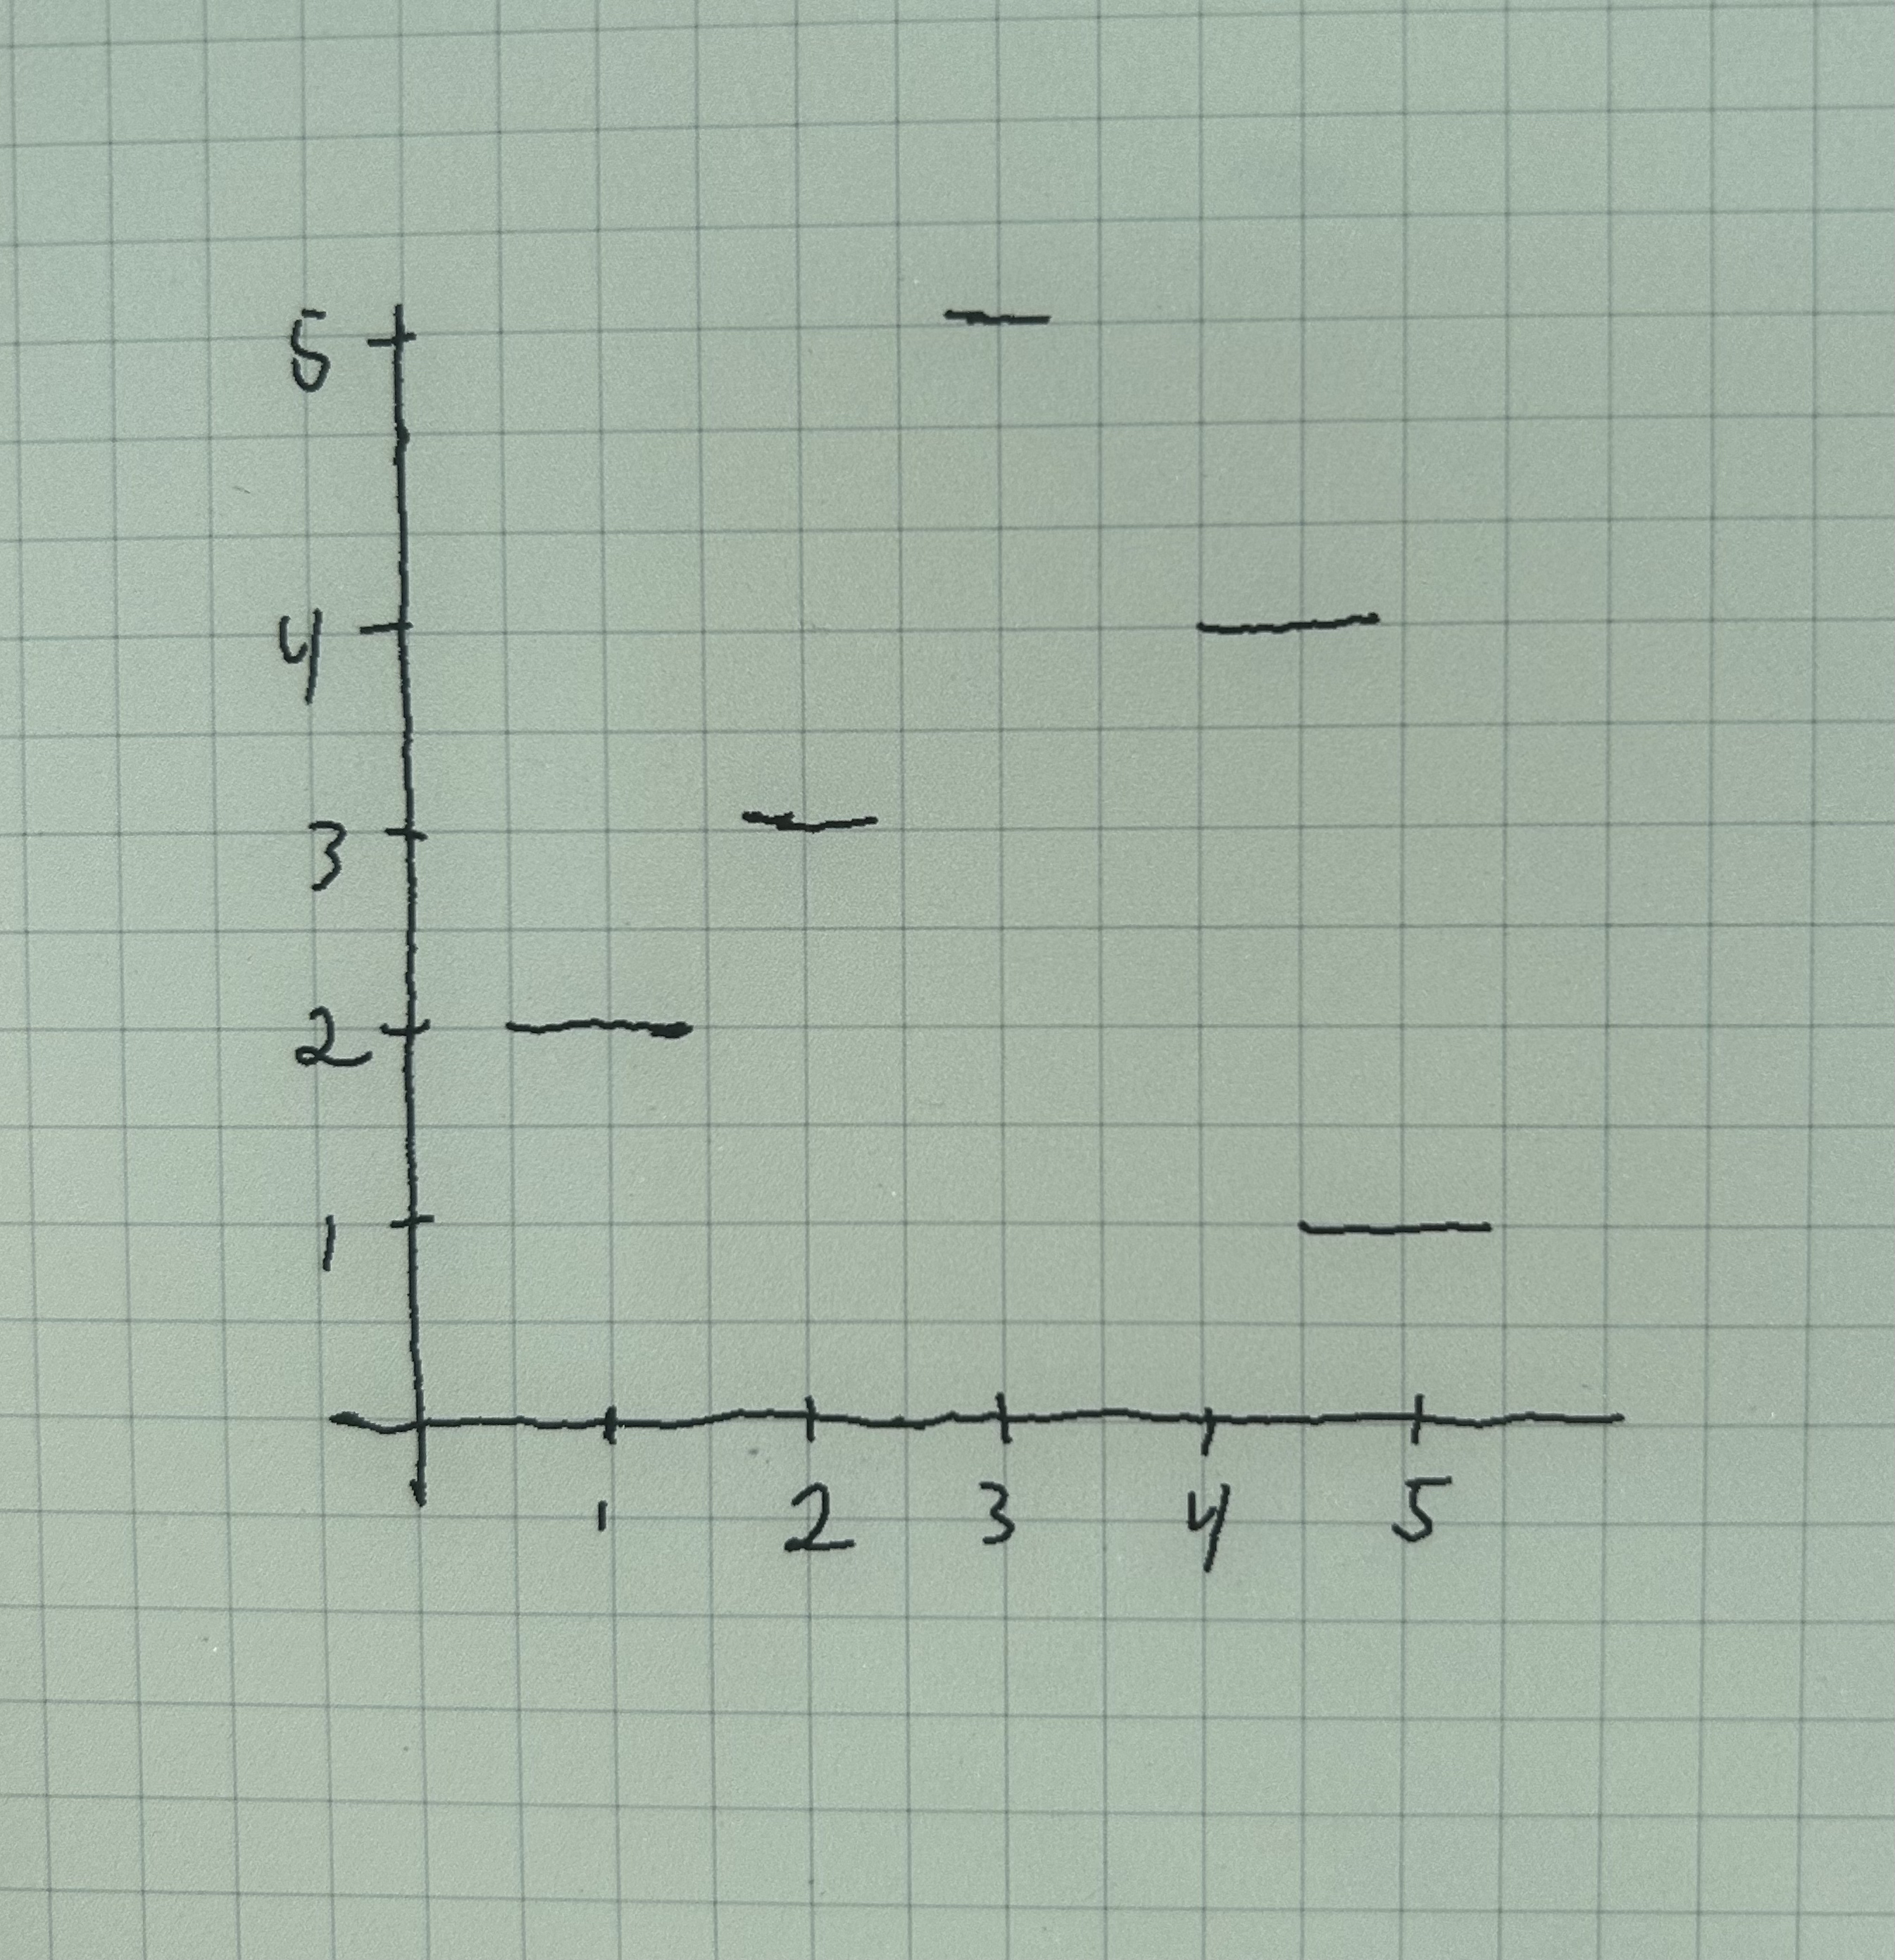
\includegraphics[scale = 0.1]{./Figures/IMG_0478.jpg}.\\

Where this graph for example represents the second shortest player walking out first, the 3rd shortest walking out 2nd, the tallest (\# 5.) walking out third, the fourth shortest walking out fourth, and the shortest walking out fifth.\\

In constructing these graphs we soon notice that in order for there to be no local minimum ever (corresponding to a player sandwiched between two players whom are both taller than him)
we can only make so many different arrangements. One way to think of it is that all our graphs need to essentially go up until they can't go up anymore, before only then falling down. This can be represented by compositions. For instance if we take a look at the same graph,
we can mark the change in height between each bar as so:
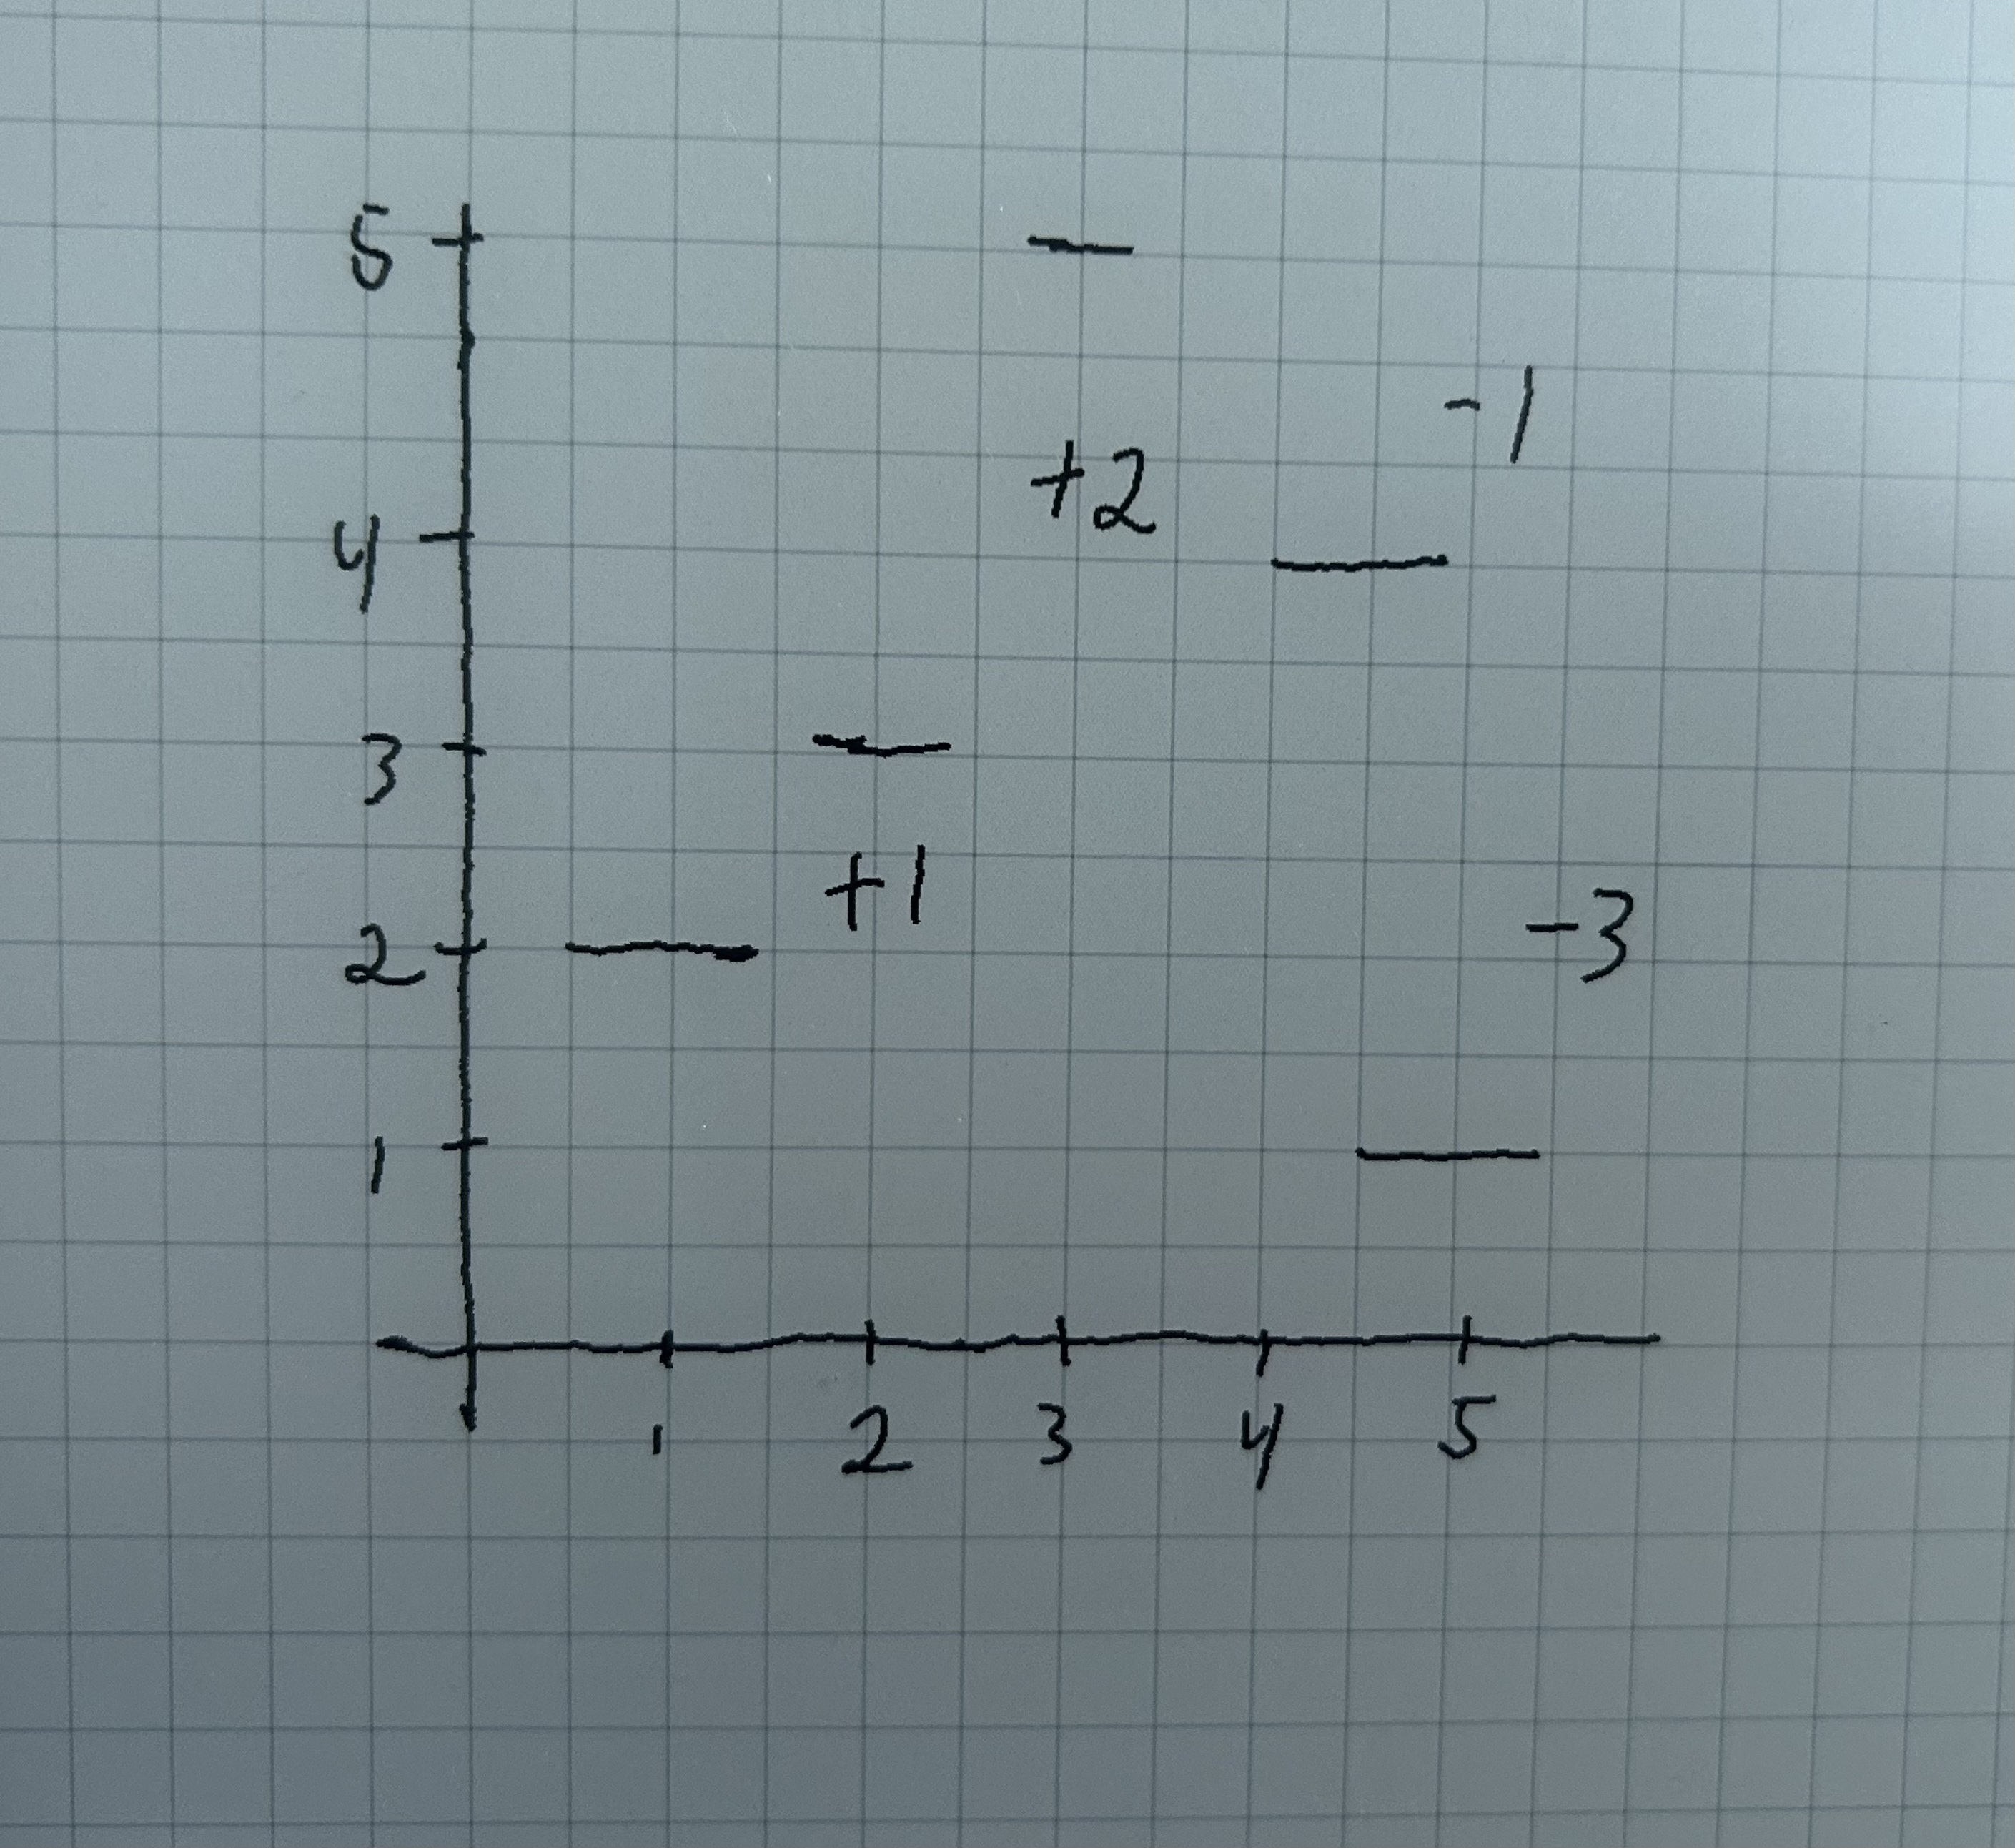
\includegraphics[scale = 0.1]{./Figures/IMG_0479.jpg}.\\

Notice however that once we decide the "up" direction of the graph, the down is already picked for us as it must be strictly decreasing. Thus the number of different ways
we can choose how to make the first part of the graph go up reduces to calculating the number of compositions of $(n-k)$ for each $k<n$. In this case that's $c(4),c(3),c(2),c(1)$ and $c(0)$. ($c(0):=1$ and coresponds to the one graph that only ever goes down).
We list the different values of $k$ and the corresponding compositions:\\

$k=1$, $5-1=4$; We have: $(1,1,1,1), (1,1,2), (1,2,1), (2,1,1), (3,1), (1,3), (4)$. Each of these corresponds to a graph and a specific way the graph increases. For example, $(1,1,2)$ corresponds with the shorest player starting (as we are in the case $k=1$), the second shortest
going in after him (1+1), the third shortest after that (1+1+1), and then the tallest player (1+1+1+2). After that, as mentioned, the graph must be strictly decreasing so we have no choice in the order any more. For $k=2$ we have $5-2=3$ so we have the compositions:
$(1,1,1), (1,2), (2,1), (3)$. Once again each corresponds with a certain graph. For example, $(2,1)$ corresponds with the 2nd shortest player entering first (as we are in the case $k=2$), then the fourth shortest (2+2),then the tallest (2+2+1). In another example, $(3)$ corresponds to the second player going first, then
the tallest after that (2+3=5). For the case $k=3$ we have $5-3=2$ so our compositions are (1,1) and (2). For the case $k=4$ we have $5-4=1$ so the only compositions we have are $(1)$.\\

Finally, as mentioned the case $k=5$ corresponds to the number of compositions for the integer 0, which we define to be 1, as it corresponds to the fifth player (i.e. tallest player) starting (and so subsequently the rest strictly decreasing).\\

We count the number of compositions we end up with and reach 16.\\

For general $n$ there are:
\begin{align*}
    &\sum_{k=1}^n c(n-k)\\
\end{align*}
where $c(x)$ is the number of compositions of $x$.\\

We can simplify this further though as the number of compositions $x$ has is $2^{x-1}$ for positive $x$ and definted to be 1 if $x$ is 0.\\

One can justify this in a number of ways though one way the author has seen is as follows. Think of each number as a series of 1s to be added.
Between each 1 you can either add a slash or a plus. Plus indicates that the composition has melded those two 1s into a new number, a slash indicates we have not done that and left it as a one instead.
For example one composition of 4 is (2,1,1). This can be represented as:\\
1 + 1 / 1 / 1. There are $n-1$ gaps between the 1s and two possible options to fill them so we have $2^{n-1}$ possibilities.\\

Thus our formula for general $n$ becomes:
\begin{align*}
    \sum_{k=1}^{n-1}2^{n-k-1} + 1.
\end{align*}

\end{problem}

\begin{problem}
    \ \\
    The answer is: $\frac{ {9\choose 3} \cdot {6 \choose 3} }{3!} = 280$.\\
    \\
    We choose the three police officers from the 9 total, then from the remaining 6, choose the next 3. The last three are picked by default.
    However since the order of the patrols don't matter, this overcounts by a factor of 3!. Thus we divide by 3!.
\end{problem}

\begin{problem}
    \ \\
    Once again we will instead ask how many numbers less than 1,000,000 don't contain the digit 2.
    That means for each of the 6 digits we have 9 different options of the number it could be (0-9 excluding 2). This leads to:
    $9^6$ total numbers less than 1,000,000 that don't contain 2. Subtract that from a million to get the number of numbers less than 1,000,000
    which contain two:
    \begin{equation*}
    1,000,000-9^6 = 468,559.\\
    \end{equation*}
\end{problem}

\begin{problem}
    We will prove the identity by first multiplying the left hand side by $\frac{n+1}{n+1}$. This yields the following:
    \begin{align*}
        &\sum_{k=0}^n \frac{1}{k+1} {n\choose k}\\
        &=\frac{n+1}{n+1}\left(  \sum_{k=0}^n \frac{1}{k+1} {n \choose k} \right)\\
        &=\frac{1}{n+1}\sum_{k=0}^n\frac{n+1}{k+1}{n\choose k}\\
        &=\frac{1}{n+1}\sum_{k=0}^n \frac{n+1}{k+1} \left( \frac{n!}{\left( n-k \right)!k!}  \right)\\
        &=\frac{1}{n+1} \sum_{k=0}^n \frac{(n+1)!}{(n-k)!(k+1)!}\\
        &=\frac{1}{n+1}\sum_{k=0}^n \frac{(n+1)!}{(n+1-(k+1))!(k+1)!}
    \end{align*}

    If we then let $s=k+1$ we have:
    \begin{align*}
        &=\frac{1}{n+1} \sum_{s=1}^{n+1} {{n+1}\choose s}\\
        &=\frac{1}{n+1} \cdot \left(  \sum_{s=0}^{n+1} {{n+1}\choose s} - 1 \right)
    \end{align*}
    As $\sum_{s=1}^{n+1} {{n+1}\choose {s}}$ is all possible subsets of an n+1-size set except for the empty set.
    So we subtract 1 from $\sum_{s=0}^{n+1} {{n+1}\choose s}$ to represent the exclusion of the empty set as a possible subset.
    We then can rewrite the last line as:
    \begin{align*}
        &\frac{1}{n+1}\left( 2^{n+1} -1  \right). &\qedsymbol
    \end{align*} 
\end{problem}
\end{document}